\section{Make people aware of how much money, time, climate they are using on commuting}
\label{sec:make-people-aware-of-how-much-money-time-climate-they-are-using-on-commuting}

A study from Denmark’s statistic clearly shows that out of the around three million people in the workforce only
185 thousand people doesn't commute to work.
This means that \(93.88\,\%\) of the working population commute to work in Denmark~\cite{erhvervspendling2021}.

People are generally uninformed about how much emissions they are helping to produce while travelling in their
desired commuting option.
The desired preference of the commuting can change the way people commutes.
A study made in 2021 on commuting showed which transport option users would pick depending on what their preferences
were.
In this study, we can clearly see that public transport is preferred when the priority is saving time, cost or being
environmentally friendly while walking or cycling were more preferred when health was the priority~\cite{spark2023}.

This is interesting because if people had the opportunity to select either economy, time or sustainability as a
preference when commuting they could use alternative transport options.
Furthermore, this could possibly promote sustainable commuting.
This may be important as sustainable living is becoming more trending than ever.
This may be a direct result of people becoming more aware of how their choices can have an effect on the environment they
live in.

Research done by Capgemini research shows a correlation between sustainability and significant business benefits.
This means that customer loyalty and revenue increases by having a focus on being sustainable~\cite{capgemini2020}.
The enlarged focus on sustainability stems from the new youth, as they prioritize sustainability more than millennials.
% Ovenstående sætning mangler reference.

Commuting can also influence mental health and well-being as it can cause an increase in stress level.
One study suggests that one of the factors increasing stress levels is that the commuters have a difficulty in
appreciating their way of commuting.
% Hvad betyder ovenstående sætning??

The author furthermore explains that the governments must prioritize what the commuters prefer.
These workers can have an incline in stress levels as they have deadlines and specific meeting times that need to be
reached in time~\cite{koslowsky2013}.
By this we can derive that having the opportunity to travel to your destination as fast as possible can be beneficial
for the health.

Another study on 208 people who were rail commuters in New York showed that the longer time that they commuted the more
their cortisol level increased.
This means that time duration of commuting is an important factor for some users.
Therefore, it is essential that people commuting can have an influence on time spent commuting.

Another critical aspect is how commuting effect the economy of people.
A study shows that the average American citizen spends \SI{8466}[\$]{} on co commute expenses.
% Hvad er co commute?
There is a different cost involved in the commute depending on which transport options are used.
For example, \(76\,\%\) of commuters use their personal vehicle~\cite{bankrate2023}.
% Mangler reference på ovenstående tal.
They may also have some extra expenses besides just the buying price of the car.
The average driver spends \SI{1771}[\$]{} on full car insurance and furthermore they spend money on car maintenance
and occasionally after 5000 miles they need to get their vehicles' oil changed.
This could be a challenge as research shows that 1 out of 3 drivers can't afford sudden unexpected car repairs.
The study also suggests that using public transport, bike or scooter to work will cost less~\cite{bankrate2023}.
This change could be difficult as commuting in a personal vehicle could be much more time efficient.

The same study showed that the working poor who commuted by public transport spend \(10\,\%\) of their income on
commuting compared to \(21\,\%\) when commuting in their car.
The working poor prefer saving money because this means they can spend a larger portion of their income on other
relevant expenses like food, healthcare, household supplies and saving for the future.
From this, it is apparent that especially the poorer people would prefer having the opportunity to
commute by cost preferences.
This could improve their economy as the working poor tend to use the least expensive options of commuting, like
carpooling, van pooling, biking, walking and public transport.
Comparing this to people with higher income they are more inclined to spend more on commuting~\cite{bankrate2023}.

% textidote: ignore begin
% TODO Reference figure in a more meaningful way, as it is not neccesary to include in the current state of the analysis
\begin{figure}
    \centering
    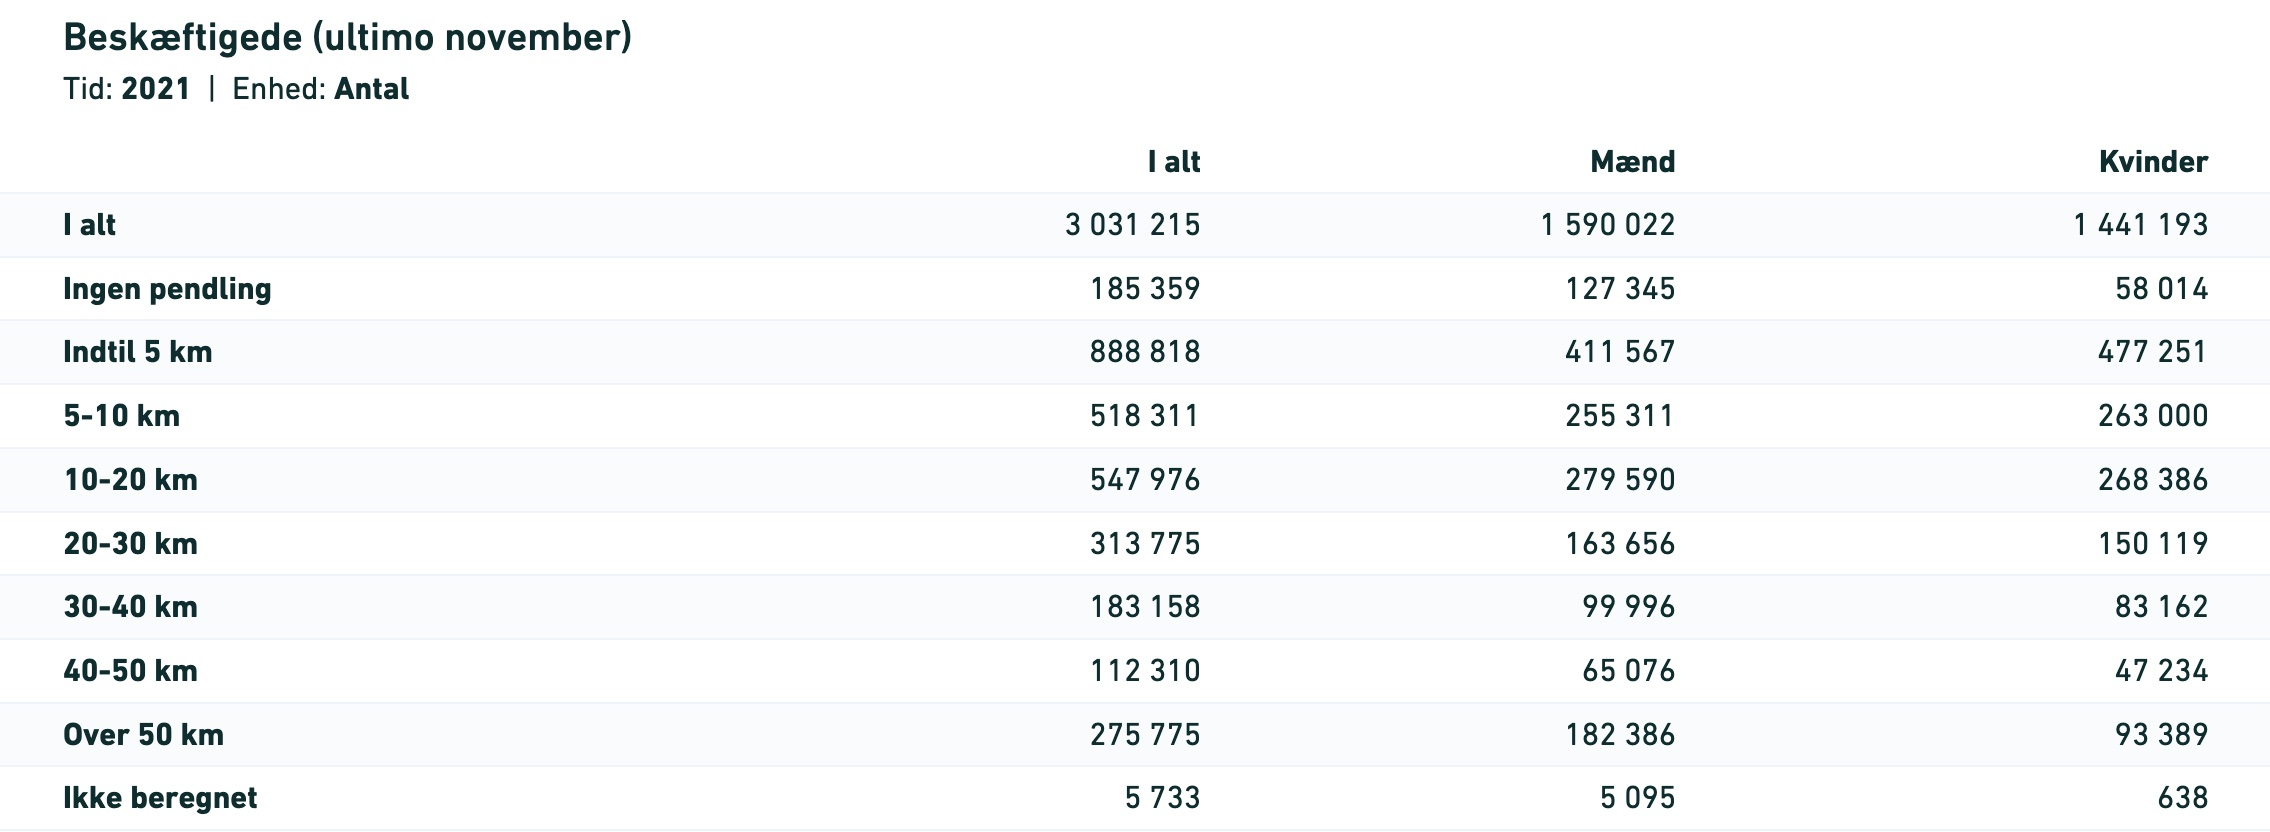
\includegraphics[width=\textwidth]{stats}
    \caption{A picture of a gull.}
    \label{fig:figure}
\end{figure}

% TODO Reference figure in a more meaningful way, as it is not neccesary to include in the current state of the analysis
\begin{figure}
    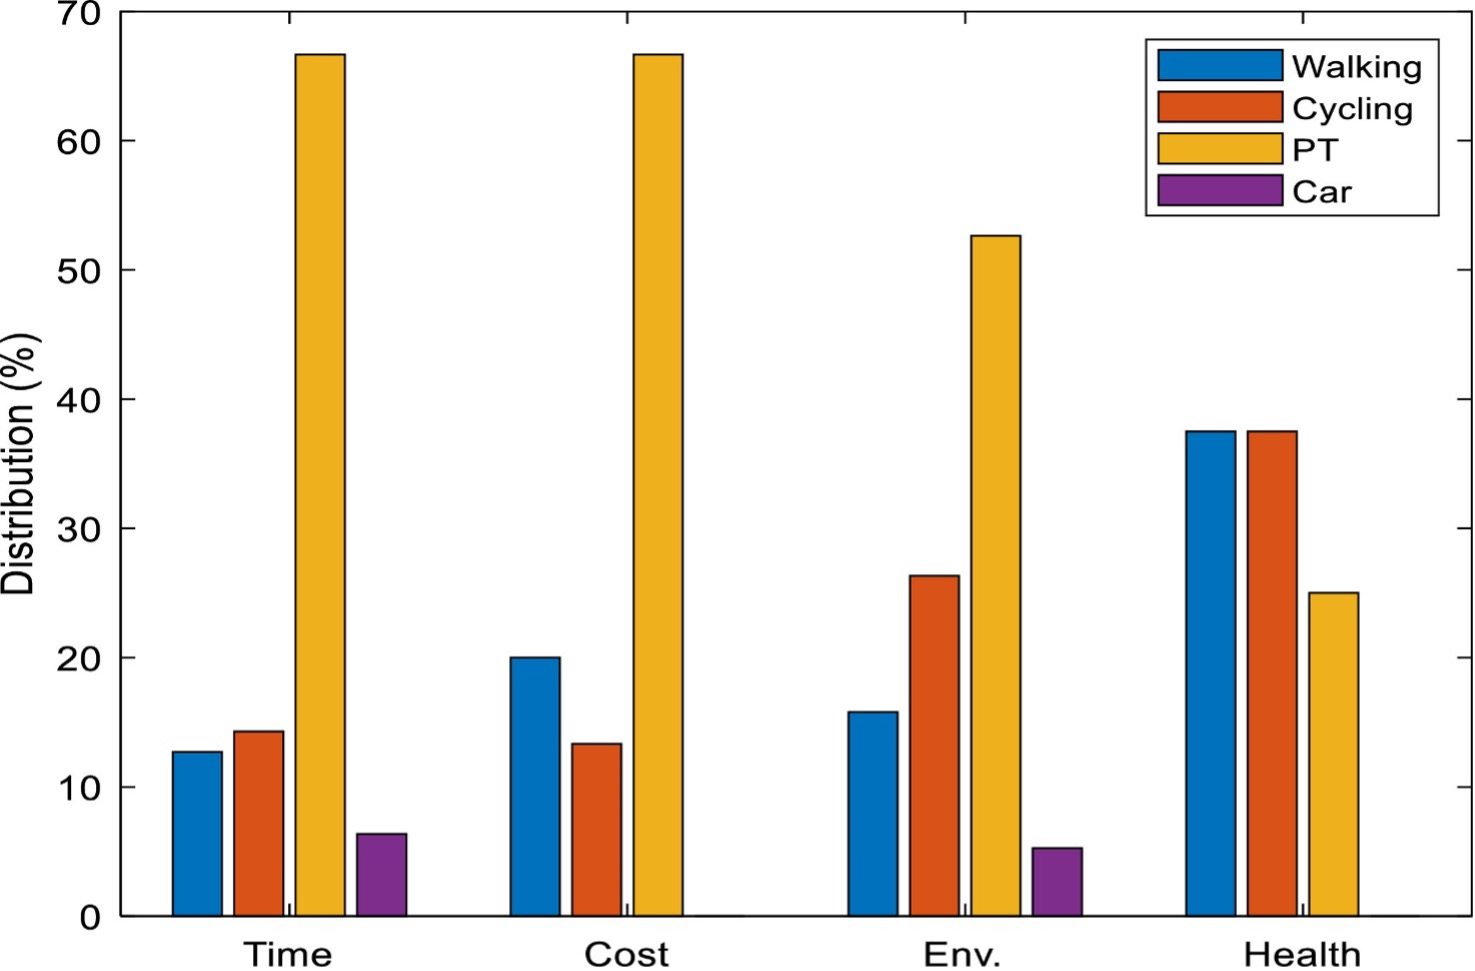
\includegraphics[width=\textwidth]{stats-2}
    \caption{A picture of a gull.}
    \label{fig:figure2}
\end{figure}
% textidote: ignore end
